\section{Concepts and Definitions}
%
\label{sec:concepts}
%
\subsection{Running Example}
%
In this paper, we use the three-tank system shown in
figure~\ref{fig:three_tanks}. The three tanks are denoted as $T_1$,
$T_2$, and $T_3$. They all have the same area $A_1 = A_2 = A_3 =
3~[\textrm{m}^2]$. The three tanks are indestructible and of infinite
height, so no overfills or anything like that happens (the experiment
is idealized). The experiments is performed on a planet similar to
ours where $g = 10$ and the liquid is ``pure'' water with density
$\rho = 1$.
%
\begin{figure}[htb]
  \centering
  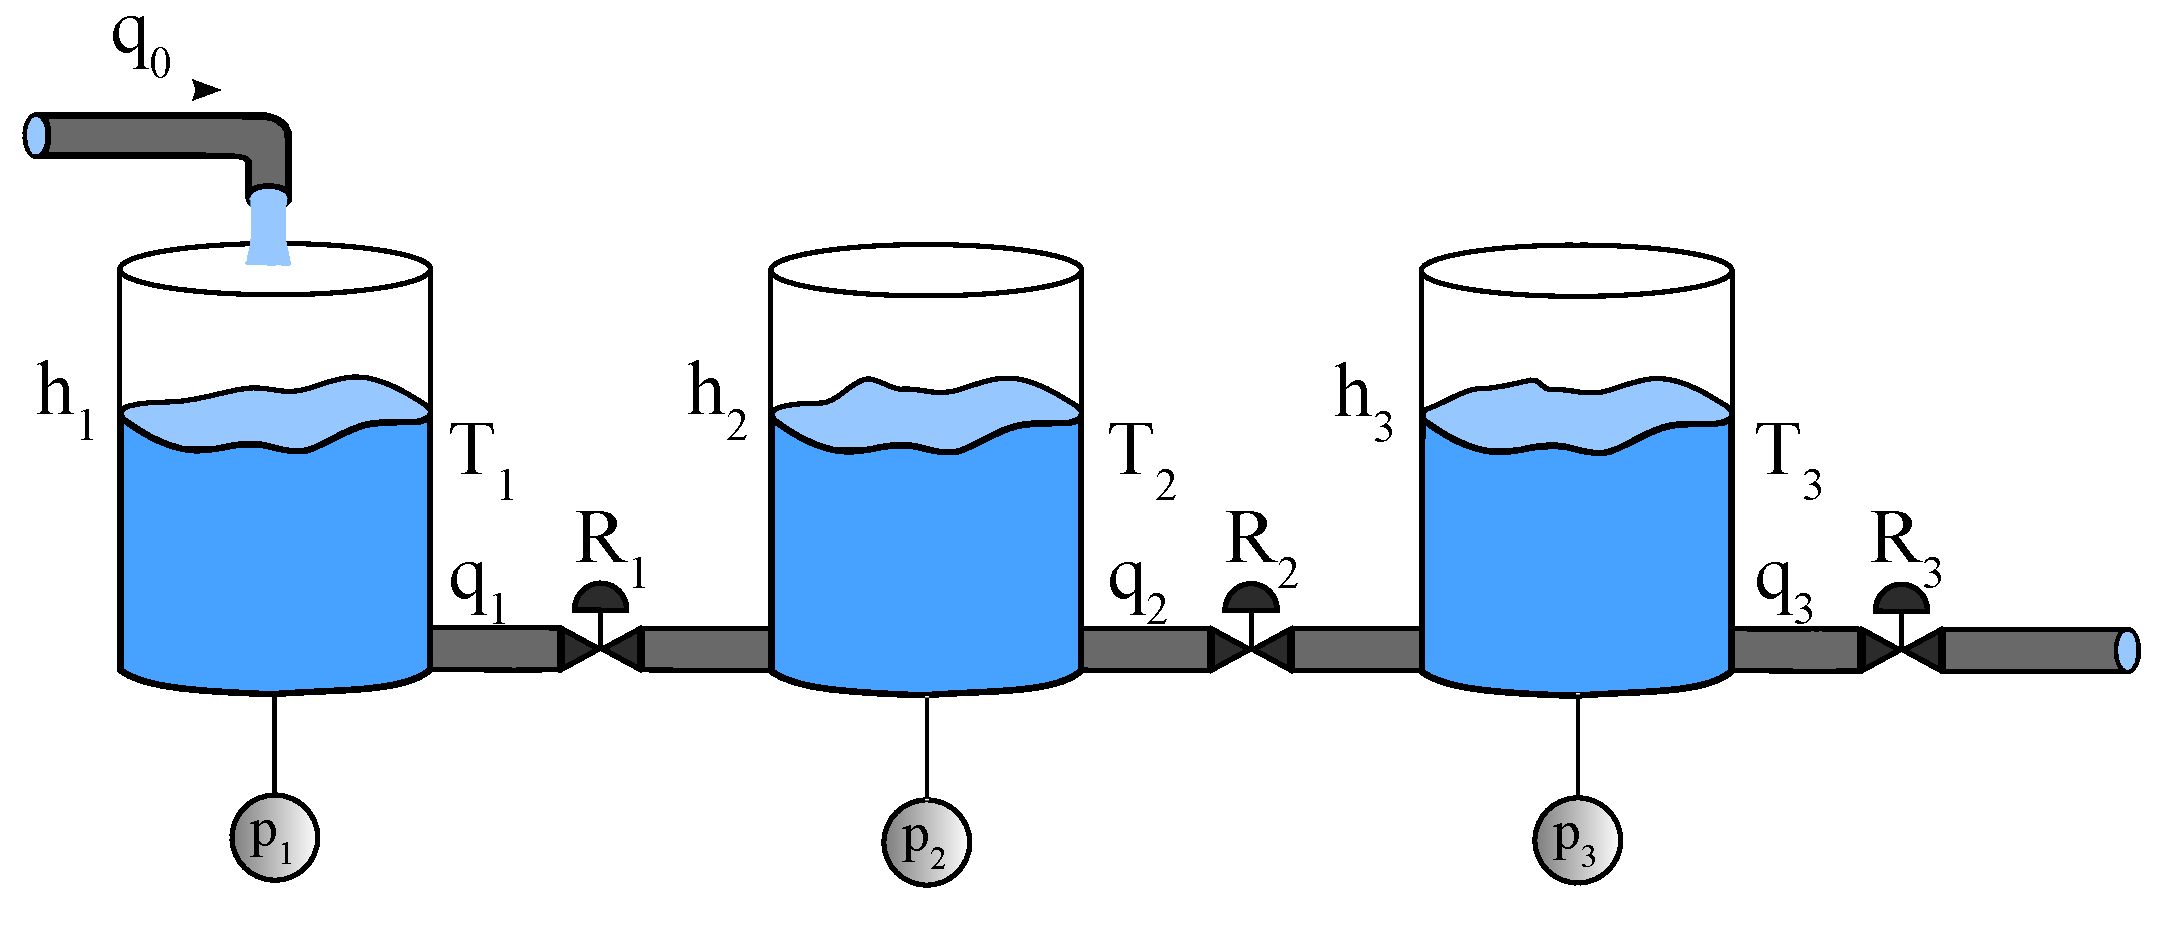
\includegraphics[width=1\columnwidth]{3-tanks}
  \caption{Diagram of the three-tank system.}
  \label{fig:three_tanks}
\end{figure}
\par\noindent
%
Tank $T_1$ gets filled from a pipe $q_0$ with a constant flow of
$0.75~[\textrm{m}^3/\textrm{s}]$. It drains into $T_2$ via a pipe
$q_1$. The liquid level is denoted as $h_1$. There is a pressure
sensor $p_1$ connected to $T_1$ that measures the pressure in Pascals
[Pa]. Starting from the Newton's (and Bernouli's) equations and
manipulating them (the actual derivation is trivial and irrelevant in
this paper) we derive the following Ordinary Differential Equation
(ODE) that gives the level of the liquid in $T_1$:
%
\begin{eqnarray}
%
\frac{d h_1}{dt} = \frac{q_0 - k_1 \sqrt{h_1}}{A_1}\label{eq:ode1}
%
\end{eqnarray}
%
In eq.~\ref{eq:ode1}, the coefficient $k_1$ is the product of the
cross-sectional area of the tank $A_1$ and the area of the drainage
hole and $\sqrt{2g}$ and the friction/contraction factor of the
hole. We emphasize the use of $k_1$ because, later, we will be
``diagnosing'' our system in term of changes in $k_1$. Consider a
physical valve $R_1$ between $T_1$ and $T_2$ that constraints the flow
between the two tanks. We can say that the valve changes
proportionally the cross-sectional drainage area of $q_1$ and hence
$k_1$. The diagnostic task will be to compute the true value of $k_1$,
given $p_1$, and from $k_1$ we can compute the actual position of the
valve $R_1$.
%
The water levels of $T_2$ and $T_3$, denoted as $h_2$ and $h_3$
respectively, are given by:
%
\begin{eqnarray}\label{eq:tank1}
%
\frac{d h_i}{dt} = \frac{k_{i - 1} \sqrt{h_{i - 1}} - k_i \sqrt{h_i}}{A_i},
%
\end{eqnarray}
%
where $i$ is the tank index ($i \in \{2, 3\}$).
\par
Let us say that $k_1 = 0.25$, $k_2 = 0.5$, and $k_3 = 0.75$ (these
values have no physical meaning, we have chosen them to produce
``nice'' simulation results).
\par
Finally, we turn the water level into pressure:
\begin{eqnarray}
p_i = \frac{g\,h_i\,A}{A} = g\,h_i
\end{eqnarray}
where $i$ is the tank index ($i \in \{1, 2, 3\}$).
\par
It is assumed that the initial water level in the three tanks is zero.
%
\subsection{Definitions}

This section introduces our notation and definitions.

%----------------------------------
\subsubsection{Model Classes}
%----------------------------------

In this article we examine several different  types of model for simulation, including dynamical, linear, and qualitative.
For our models, we consider three classes of variables:
$\vec{x}(t)$ is the state variable vector, $\vec{u}(t)$ is the input variable vector, and $\vec{y}(t)$ is the observation vector.
$\vec{\omega}(t)$ is a disturbance vector.

\begin{definition}[Non-Linear Dynamical Model $\Phi_D$]
We write the dynamical equations for a model in state-space form using
\begin{eqnarray}\label{dyn-model}
%\frac{d \vec{x}(t)}{dt} & = & \psi (\vec{x}(t)) + \vec{u}(t))\\
\dot{\vec{x}}(t) & = & \psi (\vec{x}(t)) + \vec{u}(t))\\
\vec{y}(t) & = & \gamma (\vec{x}(t)), \vec{u}(t)),
\end{eqnarray}
where $\psi$ and $\gamma$ are non-linear functions.
%---------------
\end{definition}

\begin{definition}[Linear Dynamical Model $\Phi_L$]
We write the linear dynamical equations for a model in state-space form using
\begin{eqnarray}\label{linear-model}
\dot{\vec{x}}(t) & = & \mathbf{A} \vec{x}(t) + \mathbf{B} \vec{u}(t)) + \mathbf{C} \vec{\omega}(t) +  \vec{\omega}(t)\\
\vec{y}(t) & = & \mathbf{D} (\vec{x}(t)),
\end{eqnarray}
where $\mathbf{A}, ~ \mathbf{B},~\mathbf{C}$ and $\mathbf{D}$ are linear matrices.
%---------------
\end{definition}

\begin{definition}[Qualitative Model $\Phi_Q$]
We write the dynamical equations for a model in state-space form using
\begin{eqnarray}\label{qual-model}
\dot{\vec{x}}(t) & = & \upsilon (\vec{x}(t)) + \vec{u}(t))\\
\vec{y}(t) & = & \mu (\vec{x}(t)), \vec{u}(t)),
\end{eqnarray}
where $\upsilon$ and $\mu$ are  functions from the set of reasonable functions $f$ such that $f' > 0$ on the interior of its domain \citep{kuipers1994composition}.
%---------------
\end{definition}

\begin{definition}[Boolean Model $\Phi_B$]
We write the dynamical equations for a model in state-space form using
\begin{eqnarray}\label{boolean-model}
\frac{d \vec{x}(t)}{dt} & = & \upsilon (\vec{x}(t)) + \vec{u}(t))\\
\vec{y}(t) & = & \mu (\vec{x}(t)), \vec{u}(t)),
\end{eqnarray}
where $\upsilon$ and $\mu$ are  functions from the set of reasonable functions $f$ such that $f' > 0$ on the interior of its domain \citep{kuipers1994composition}.
%---------------
\end{definition}

This definition of model identifies only a single set of \textit{ideal} conditions under which the model applies. More generally, real-world systems require models that can simulate over multiple possible modes, where a mode is a set of conditions under which the system is operating. For example, a car can drive in a range of gears (forward and reverse), and the dynamics of each gear are different and require different simulation models. In addition to these nominal modes, we can identify a set of failure modes, where the system is operating given some level of degradation. 

With this general notion in mind, we can define a system now to have a set of equations $\cal E$ associated with a mode $M$, using the pair $(M,{\cal E}_M)$. The generalized notion of model now becomes $({\cal M},{\cal E})$, where the equations can be dynamical, linear, qualitative or Boolean.
We distinguish two classes of mode, nominal modes ${\cal M}_N$ and failure modes ${\cal M}_F$.


%----------------------------------
\subsubsection{Simulation/Diagnosis Problem}
%----------------------------------

In the following, we assume that we have a system model $\Phi$ based on a real system $\cal S$, together with measured data $\alpha$ from $\cal S$.

\begin{definition}[Simulation Problem]
Given 
%a system model $\Phi$, 
initial conditions $\cal I$, and measured data $\alpha$, simulation aims to specify a model $\Phi$ that minimises a difference metric (e.g., sum of squared error) between the simulation output $\Phi(\alpha, {\cal I})$ and $\alpha$.
%initial vectors
\end{definition}

%%%%%%%%%%%%%%%%%%%%%%%%%%%%%%



\begin{definition}[Diagnosis Problem]
simulation model, sensor data
\end{definition}

\begin{definition}[Diagnosis Model]
simulation model, sensor data
\end{definition}

\begin{definition}[Diagnosis $\d$]

\end{definition}


%----------------------------------
\subsubsection{Ensemble Diagnosis}
%----------------------------------



We assume that we have a family of system models $\Phi = \{\phi_1,...,\phi_n\}$.
Given a system observation $\mathbf{\alpha}$, model $\phi_i$ generates a class label (diagnosis) $\d_i$, together with a probability that the diagnosis is correct, $\psi_i(\d|\mathbf{\alpha})$. We call $\psi_i(\d|\mathbf{\alpha})$ the prediction model for  $\phi_i$.


We adopt an approach in which we use classification ensembles to produce class probability estimates. 
\begin{definition}[Ensemble Prediction $\bar{\psi}(\d|\mathbf{\alpha})$]
We have a prediction model $\psi_i(\d|\mathbf{\alpha})$, an estimate of the probability of class $\d$ given input $\mathbf{\alpha}$. For a set of these, $i = {1...I}$, the ensemble probability estimate is given by
\begin{equation}
\bar{\psi}(\d|\mathbf{\alpha})~=~\sum_{i=1}^I \zeta_i  \psi_i(\d|\mathbf{\alpha}).
\end{equation}
\end{definition}

The simplest approach is to adopt uniform averaging of the probability estimates, in which case we have $\zeta_i = \frac{1}{T}, ~\forall T$.
Using non-uniform weights is potentially more accurate if the classifiers have different accuracies on the data, as this could provide a lower error solution than a uniform combination.
However, applying non-uniform weights is challenging theoretically and practically.
Typically, only relatively small gains may be achieved when estimating the $\vec{\zeta}$ parameters without overfitting (see \citep{kuncheva2004combining}, p282).


%===============================================
\subsubsection{Metrics}
%===============================================
%5. Metrics:
%        5.1. simulation accuracy - error
%        5.2. diagnostics: false positives, false negatives, isolation time, computational resources, if you wish component cost (I wouldn't go there)


In order to compare the different models and their performance, we need to specify a set of metrics. We group our metrics in terms of (a) diagnostics accuracy, (2) simulation accuracy, and (3) model costs.

\subsubsection{Simulation Accuracy}

\begin{definition}[Simulation Accuracy]
Given a system model $\Phi$, 
initial conditions $\cal I$, and measured data $\alpha$, simulation accuracy is measured using a difference metric $\Delta$ between the simulation output $\Phi(\alpha, {\cal I})$ and $\alpha$.
\end{definition}

$\Delta$ can be measured using a variety of methods, e.g., sum of squared error.

\subsubsection{Diagnostics Accuracy}


false positives, false negatives, isolation time, computational resources



\subsubsection{Model Costs}

Models are inherently expensive to create, and it is critical to define costs of creating models. The most common  framework is to create a model library from which task-specific models can be developed. The challenge is to define a component library with components of appropriate fidelity. 

Representing the notion of appropriate fidelity is extremely difficulty. One of the best attempts to define this is the notion of \textit{proper model} \cite{??}.


We assume that a component would have a generic set of parameters, which would be tuned when a system-specific model is constructed.


\begin{definition}[Component Model Cost]
????
\end{definition}

\begin{definition}[System Model Cost]
????

components + parameter estimation

\end{definition}













